\documentclass[a4paper,article]{article}

% Шрифты
\usepackage{fontspec}
\usepackage[14pt]{extsizes}
\setmainfont{Times New Roman}

% Языки
% Русский обязательно идёт вторым. Иначе не работают переносы
\usepackage[english, russian]{babel}

% Параметры страницы
\usepackage[left=3cm, top=2cm, right=1.5cm, bottom=2cm]{geometry}
\usepackage[onehalfspacing]{setspace}

% Параметры текста
% По умолчанию LaTeX не делает отступ после \section. Вроде как оно и не надо, но в тексте ВКР пусть лучше будет. В требованиях отступ описан. Этот пакет своим наличием добавляет этот отступ
\usepackage{indentfirst}
% По умолчанию абзацный отстум меньше требуемого. Задаём конкретный
\setlength{\parindent}{1.25cm}

% Ссылки
\usepackage{color}
\definecolor{Black}{RGB}{0,0,0}
% Без colorlinks вокруг ссылок появляются рамки, недопустимые в ВКР
% Если не зачернить ссылки, то в оглавлении и в других местах будут яркие цвета
\usepackage[colorlinks, allcolors=Black]{hyperref}
% Шрифт для URL
\urlstyle{rm}

% Пункты оглавления
\usepackage{titlesec}
\titleformat{\section}
{\centering\normalfont\bfseries}{\thesection. }{0em}{}
\titleformat{\subsection}
{\centering\normalfont\bfseries}{\thesubsection. }{0em}{}
\titleformat{\subsubsection}
{\centering\normalfont\bfseries}{\thesubsubsection. }{0em}{}
\titleformat{\paragraph}
{\normalfont\normalsize\bfseries\centering}{\theparagraph. }{0em}{}
% Список использованных источников
\addto\captionsrussian{\def\refname{Список использованных источников}}

% Нумерация
\setcounter{secnumdepth}{4}

% Таблицы
\usepackage{multicol}
\usepackage{xltabular}

% Перечисления
\usepackage{enumitem}

% Картинки
% Вставка картинок правильная
\usepackage{graphicx}
% "Плавающие" картинки
\usepackage{float}
% Обтекание фигур (таблиц, картинок и прочего)
\usepackage{wrapfig}
% Папка для всех картинок файла
\graphicspath{{images/}}
% Точка в конце названий объекта вместо двоеточия. Например, для Рисунков
\usepackage[labelsep=period]{caption}
% Вместо 'Рис. 1' чтобы было 'Рисунок 1'
\makeatletter
\renewcommand{\fnum@figure}{Рисунок \thefigure}
\makeatother

\begin{document}
    \begin{titlepage}
        \begin{center}
            {\bfseries Министерство науки и высшего образования Российской Федерации \\
            Федеральное государственное автономное образовательное учреждение \\
            высшего образования \\
            <<КАЗАНСКИЙ (ПРИВОЛЖСКИЙ) ФЕДЕРАЛЬНЫЙ УНИВЕРСИТЕТ>>}
        \end{center}

        \begin{center}
            ИНСТИТУТ ВЫЧИСЛИТЕЛЬНОЙ МАТЕМАТИКИ И ИНФОРМАЦИОННЫХ ТЕХНОЛОГИЙ
        \end{center}

        \begin{center}
            КАФЕДРА АНАЛИЗА ДАННЫХ И ТЕХНОЛОГИЙ ПРОГРАММИРОВАНИЯ
        \end{center}

        \begin{center}
            Направление: 09.03.03 – Прикладная информатика
        \end{center}

        \vspace{0mm}

        \begin{center}
            ВЫПУСКНАЯ КВАЛИФИКАЦИОННАЯ РАБОТА \\
            {\bfseries СИСТЕМА ЗАПИСИ НА ПРИЁМ В МЕДИЦИНСКОЕ УЧРЕЖДЕНИЕ}
        \end{center}

        \vfill

        \begin{xltabular}{\textwidth} {
                >{\hsize=0.5\hsize} X
                >{\hsize=0.5\hsize} X }
            \bfseries{Работа завершена:} & \\
            Студент 4 курса & \\
            группы 09-951 & \\
            <<\underline{\hspace{1cm}}>>\underline{\hspace{3cm}} 2023г. & \underline{\hspace{3cm}}/Колесников Д.А. \\
            & \\
            \bfseries{Работа допущена к защите:} & \\
            Научный руководитель & \\
            старший преподаватель & \\
            <<\underline{\hspace{1cm}}>>\underline{\hspace{3cm}} 2023г. & \underline{\hspace{3cm}}/Еникеев И.А. \\
            & \\
            \multicolumn{2}{l}{Заведующий кафедрой анализа данных} \\
            и технологий программирования & \\
            <<\underline{\hspace{1cm}}>>\underline{\hspace{3cm}} 2023г. & \underline{\hspace{3cm}}/Бандеров В.В. \\
        \end{xltabular}

        \vspace{0mm}

        \begin{center}
            Казань — 2023
        \end{center}
    \end{titlepage}

    \newpage

    \setcounter{page}{2}

    \tableofcontents

    \newpage

    \section*{Глоссарий}
    \addcontentsline{toc}{section}{Глоссарий}

    \textbf{API} -- Описание способов взаимодействия одной компьютерной программы с другими~\cite{apiwikipedia}

    \textbf{CRUD} -- акроним, обозначающий четыре базовые функции, используемые при работе с базами данных: создание (create), чтение (read), модификация (update), удаление (delete)

    \textbf{HTTP} -- протокол, используемый для передачи гипертекстовых документов в Интернете

    \textbf{JSON} -- текстовый формат обмена данными, основанный на JavaScript. Представляет собой набор пар "ключ: значение"

    \textbf{URL} -- строка, используемая для идентификации ресурса в Интернете

    \textbf{Алерт} -- пользовательское уведомление, информирующее о каком-либо событии

    \textbf{База данных} -- структурированный набор данных для простого взаимодействия пользователя с ними

    \textbf{Бизнес-логика} -- часть программы, определяющая правила обработки данных. Описывает процессы организации в виде кода

    \textbf{Класс} -- шаблон для создания объектов. Определяет набор полей и методов, доступных для объекта

    \textbf{Клиент} -- система, подключающаяся к серверу для доступа к его ресурсам и услугам

    \textbf{Конечная точка} -- url, на который приложения отправляют запросы для взаимодействия с веб-сервисами

    \textbf{Массив} -- структура данных, представляющая набор идентифицируемых элементов

    \textbf{Метод} -- Блок кода, выполняющий конкретную задачу. Используется для организации кода

    \textbf{Много к одному} -- тип отношения в базе данных, когда несколько записей в одной таблице связаны с одной и той же записью в другой таблице

    \textbf{Нормализация} -- Процесс организации данных в базе данных, нацеленный на повышение её гибкости и защищённости

    \textbf{Объект} -- экземпляр класса, то есть созданная и действующая по правилам класса структура

    \textbf{Один к одному} -- тип отношения в базе данных, когда одна запись в таблице связана не более чем с одной записью в другой таблице

    \textbf{Поле} -- элемент данных, который является частью структуры, как класс или запись в базе данных

    \textbf{Разрешение экрана} -- количество пикселей, отображаемых на устройстве вывода изображения

    \textbf{РКИБ} -- ГАУЗ <<Республиканская клиническая инфекционная больница имени Агафонова>>

    \textbf{Ресурс} -- в контексте API -- единица данных или функциональности, которую можно получить через API, в иных случаях -- любой элемент, который может использоваться программой (файлы, память и так далее)

    \textbf{Сервер} -- в контексте системы - специальное приложение, обеспечивающее ресурсами другие приложения. Обрабатывает HTTP-запросы, выполняет необходимую бизнес-логику

    \textbf{СУБД} -- комплекс программ, предназначенный для создания, управления и обработки баз данных

    \textbf{Сущность (Entity)} -- объект, представляющий запись в базе данных

    \textbf{Технологический стек} -- конкретный набор технологий, используемых для разработки и запуска приложения

    \textbf{Триггер} -- в контексте базы данных -- специальная процедура, автоматически срабатывающая при заданных событиях

    \textbf{Фреймворк} -- абстрактная платформа, предоставляющая общую структуру приложения для упрощения разработки

    \newpage

    \section*{Введение}
    \addcontentsline{toc}{section}{Введение}

        Медицинской отрасли не хватает информатизации. Это устоявшаяся сфера, однако она не соответствует современности: никто не хочет стоять в очередях, вручную заполнять документы, потерять выданный рецепт. В 2018 году Правительство РФ создало национальный проект <<Здравоохранение>>, направленный на улучшение медицины. Одна из задач проекта - перенос Минздравом в электронный формат части услуг: выдача рецептов, запись к врачу, подача заявления на полис, хранение медицинских документов~\cite{natsproektzdravoohranenie}.

        На деле перевели услуги в электронный формат не везде. В России 30~000 медицинских учреждений и нужно много времени для внедрения системы в каждое из них. При этом нужно учитывать особенности каждого учреждения - то, что подойдёт больнице в Москве, может не подойти поликлинике из маленького города.

        Одно из учреждений так и не перешедших в электронный формат - Республиканская клиническая инфекционная больница имени Агафонова (далее РКИБ). Сейчас в неё активно внедряюся цифровые технологии, например - оплата услуг. Но некоторые элементы остаются прежними, в частности, запись на приём. С ней то нам и предстоит разобраться.

        \textbf{Цель:} Информатизировать запись на приём в РКИБ

        \textbf{Задачи:}

        \begin{enumerate}[nolistsep]
            \item Изучить предметную область
            \item Проанализировать существующие аналоги
            \item Составить техническое задание
            \item Спроектировать части будущей системы
            \item Реализовать спроектированные части системы
        \end{enumerate}

        \textbf{Объект исследования:} Информатизация в системе здравоохранения

        \textbf{Предмет исследования:} Запись на приём в медицинское учреждение

        \textbf{Структура:} В первой части работы анализируется предметная область и определяется необходимый функционал. Во второй главе будущая система проектируется, в третьей - реализуется. Заключительная, четвертая часть - введение готовой системы в эксплуатацию.

        \newpage

    \section{Предметная область}

    \subsection{Основные сведения}

        РКИБ специализируется на помощи с инфекционными патологиями. Сюда приходят лечиться люди с хроническими заболеваниями и те, кто хочет исследоваться на наличие болезней. Другие поликлиники направляют пациентов в РКИБ, потому что здесь предоставляется большое количество услуг: рентген, диагностика и лечение разных болезней, проведение лабораторных исследований, содержание больных в стационаре.

        В этой больнице нет живых очередей. Каждый пациент записывается на какое-то время и принимается только по записи. Нет ситуаций, когда приходят "Только спросить" или когда требуется неотложная помощь. Этим РКИБ отличается от большинства других поликлиник.

        Врачи сами задают время своего приёма. Они составляют расписание на 2 недели вперёд, но оно может и измениться, например, если врач заболел. Расписание передаётся в регистратуру, где пациентов и записывают на приём.

    \subsection{Существующие решения}

    \subsubsection{Текущее решение проблемы}\label{Текущее решение проблемы}

        На момент начала работы в РКИБ нет никакой информатизированной системы записи на приём. На каждого врача и, иногда, услугу заведена отдельная тетрадь. Пример такой тетради приведён на Рисунке~\ref{fig:Тетрадь на УЗИ+ФС}.

        \begin{figure}[h]

            \centering

            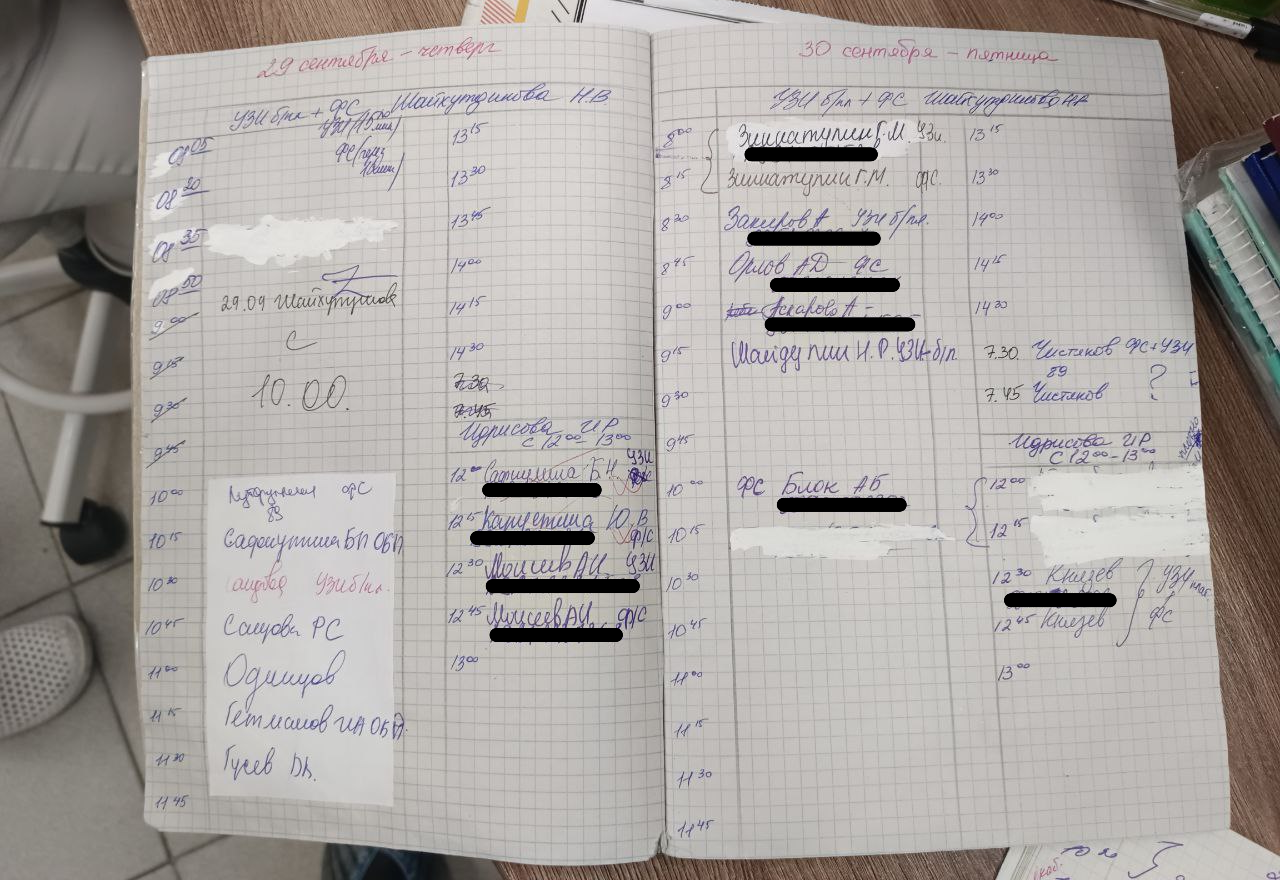
\includegraphics[width=0.8\linewidth]{Пример заполненной тетради на УЗИ+ФС. Чёрным закрашены номера телефонов.png}

            \caption{\centering Пример заполненной тетради на УЗИ+ФС. Чёрным закрашены номера телефонов}

            \label{fig:Тетрадь на УЗИ+ФС}

        \end{figure}

        Пациент, приходя в больницу, иду в регистратуру. Там его вручную записывают в тетрадь на конкретное время к конкретному врачу, вписывают его данные в тетрадь. Далее в указанное время человек приходит к врачу.
        На первый взгляд схема проста и в ней сложно допустить ошибки, но если посмотреть внимательнее, то у неё много недостатков:

        \begin{itemize}[nolistsep]
            \item \textbf{Отсутствие синхронизации.} Если пациент отменил запись, то изменение нужно сделать везде, где было упоминание о приёме.
            \item \textbf{Невозможность копирования.} Каждый врач должен несколько раз в день сверяться с записью к нему, потому что актуальная копия только в регистратуре. При составлении отчётов также требуется переносить сведения о приёме. То есть вручную переписывать сотни строк.
            \item \textbf{Невозможность обработки.} Нужно постараться, чтобы найти данные о пациенте, который приходил месяц назад. Если тетрадь поменялась, то потребуется ещё и находить архивные записи. Восстановить таким образом графики врачей задача тоже не из простых.
            \item \textbf{Дублирование информации.} В РКИБ, по словам сотрудников, много регулярных пациентов. Если кто-то приходит каждый месяц, то в тетрадях он будет записан столько раз, сколько приходил. Редко когда у человека меняется, например, отчество или дата рождения. Эти данные записываются по нескольку раз, хотя это не имеет никакого смысла.
            \item \textbf{Невозможность качественного планирования расписания.} У врачей часто меняется график работы, а в тетради строки фиксированы и ограничены. При любом изменении в графике нужно вручную найти конфликтующие пункты и изменить их.
            \item \textbf{Хранение неактуальной информации.} Человек, поменявший место работы, навсегда в какой-то из тетрадей останется на прошлом.
        \end{itemize}

        Несмотря на недостатки, РКИБ использует этот способ. Всё из-за того, что он прост для понимания, доступен и к нему привыкли. Разработанная в результате система должна быть приближена к этому, чтобы под неё не нужно было долго переучиваться.

    \subsubsection{1С:Медицина}

        <<1С:Медицина>> - решение от компании 1С. Продуманное, сделанное профессионалами, проверенное временем. Пример интерфейса на Рисунке~\ref{fig:Интерфейс 1С:Медицина}. Это мог бы быть хороший вариант, но у него тоже есть недостатки:

        \begin{itemize}[nolistsep]
            \item \textbf{Отсутствие интеграции с существующими системами.} Несмотря на то, что в РКИБ слабо информатизирована, что-то у неё уже есть. Переход на 1С означает отказ от практически всего разработано ранее, либо дополнительные затраты на интеграцию.
            \item \textbf{Избыточность.} Система нацелена на универсальность, поэтому в ней много фунцкций, не нужных этой больнице, их можно было бы упростить. Сложность системы приводит к сложности её внедрения и обслуживания.
            \item \textbf{Цена и поддержка.} Система стоит не малых денег, а поддержка будет требовать дополнительных вложений. При этом, если верить отзывам из открытых источников, поддержка и документация не всегда могут оперативно помочь.
        \end{itemize}

        \begin{figure}[h]

            \centering

            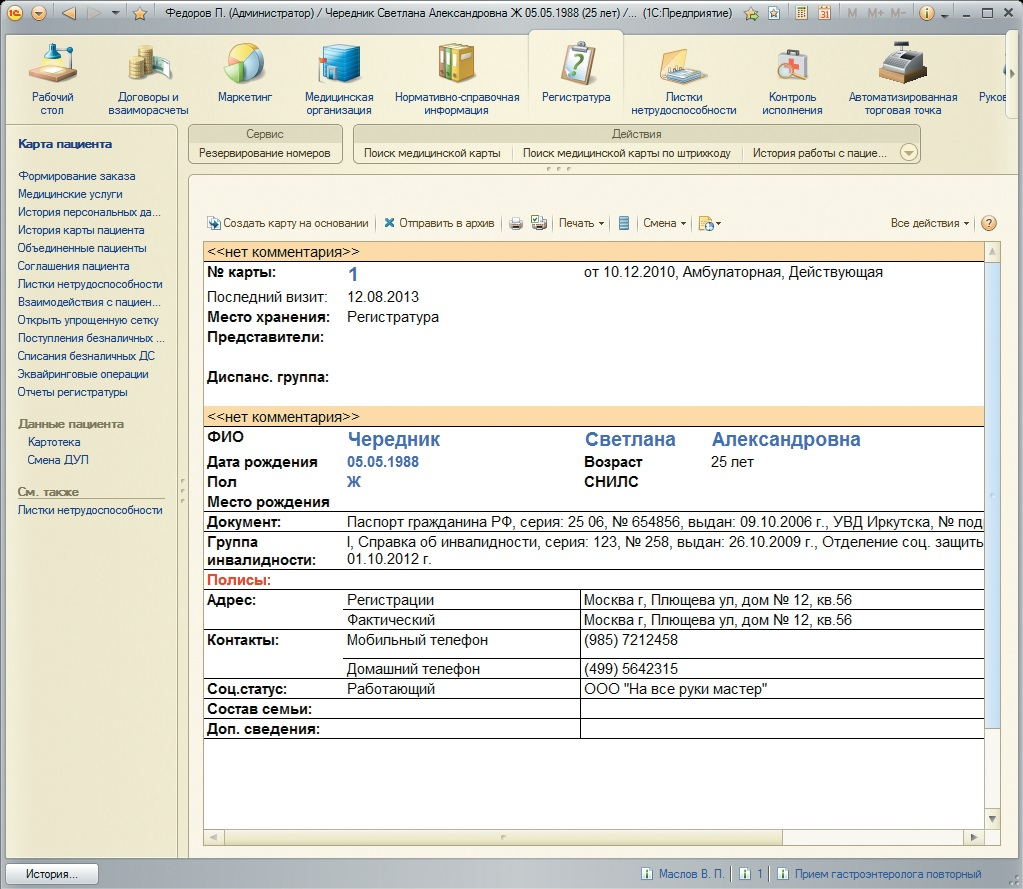
\includegraphics[width=0.6\linewidth]{Интерфейс 1С:Медицина.png}

            \caption{\centering Интерфейс 1С:Медицина}

            \label{fig:Интерфейс 1С:Медицина}

        \end{figure}

    \subsubsection{Другая предлагавшаяся система}

        Разрабатываемая система - не первая, которую хотели внедрить в РКИБ. По словам сотрудников, им уже предлагали готовое решение. Проблема в том, что система не была приспособлена к использованию в этой больнице. Она подходила обычной поликлинике, но РКИБ слишком сильно от них отличается. Здесь нет привычных участков. Обслуживаются не только жители ближайших районов, но и, во том числе, других регионов. Это помешало внедрить её в РКИБ.

        Приспособленность к работе в условиях этой конкретной больницы - важное условие для запуска системы.

    \subsection{Техническое задание}\label{Техническое задание}

        В системе выделяются 4 роли:

        \begin{itemize}[nolistsep]
            \item Пациент
            \item Доктор
            \item Регистратор
            \item Администратор
        \end{itemize}

        Каждая из них отличается требуемым функционалом. Диаграмма вариантов использования представленя на Рисунке~\ref{fig:Диаграмма вариантов использования}. Далее рассмотрим их поподробнее.

        \begin{figure}[h]

            \centering

            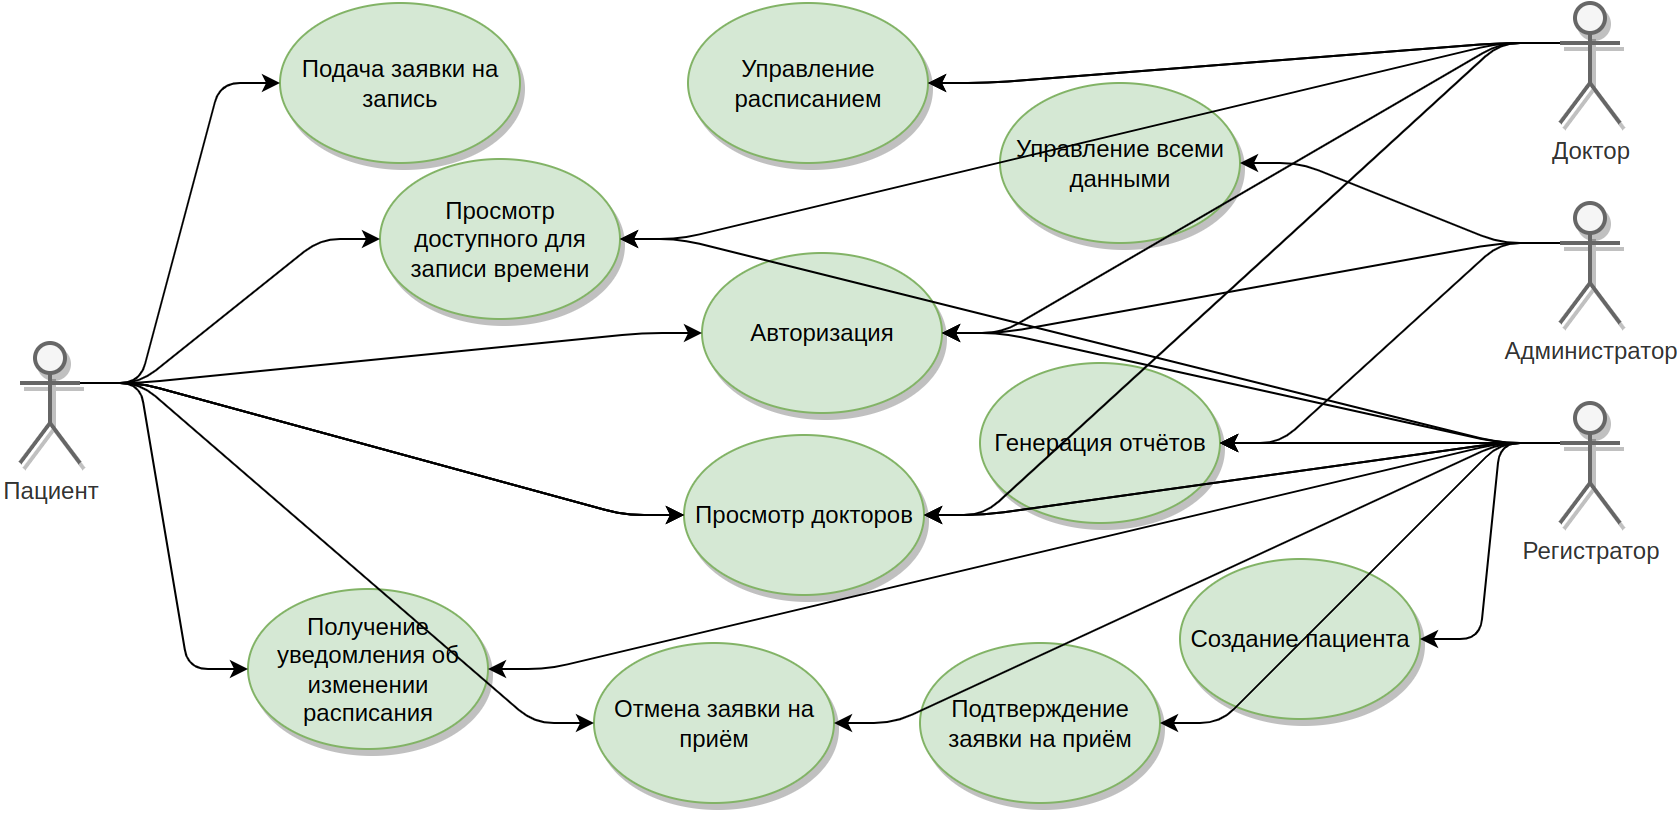
\includegraphics[width=0.8\linewidth]{Диаграмма вариантов использования.png}

            \caption{\centering Диаграмма вариантов использования}

            \label{fig:Диаграмма вариантов использования}

        \end{figure}

    \subsubsection{Функциональные требования}\label{ТЗ. Функциональные требования}

    \paragraph{Пациент}\label{ТЗ. Пациент}

    \paragraph{Доктор}\label{ТЗ. Доктор}

    \paragraph{Регистратор}\label{ТЗ. Регистратор}

    \paragraph{Администратор}\label{ТЗ. Администратор}

    \newpage

    \subsubsection{Нефункциональные требования}

    В этом разделе рассмотрим критерии, изпользуемые для оценки работы системы - характеристики производительности и некоторые атрибуты качества.

    \paragraph{Совместимость}\label{ТЗ. Интерфейс пользователя}

    Система должна корректно работать Chromium, Яндекс.Браузер, Edge версий, актуальных на начало 2023 года. Должна гарантироваться работа на экранах с разрешениями от 1024x768 до 1920x1440 для соотношения сторон 4:3, и с разрешениями 1280x720 до 1920x1080 для соотношения сторон 16:9. Указанные разрешения предполагают развёрнутость окно браузера на полный экран.

    Для каждого из вариантов использования из пункта~\ref{}

    \paragraph{Безопасность}\label{ТЗ. Безопасность}

    Использование системы должно происходить только через HTTPS. Пароли должны храниться в таком виде, чтобы из него было невозможно узнать изначальный пароль. Следовательно, не должно быть возможности восстановить пароль - только сбросить и создать новый.

    \paragraph{Производительность}\label{ТЗ. Производительность}

    Система должна корректно работать при одновременном подключении как минимум 10 пользователей без значительного снижения производительности - не более 10 секунд на запрос при условии стабильного подключения интернета 100Мбит/с.

    \pagestyle{plain}

    \newpage

    \section{Проектирование}\label{Проектирование}

    Разрабатываемая система - клиент-серверное приложение. Простейшая схема клиент-серверного приложения представлена на Рисунке~\ref{fig:Схема клиент-серверного приложения}.

    \begin{figure}[h]

        \centering

        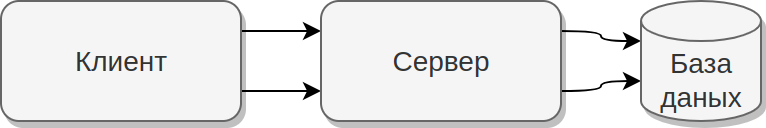
\includegraphics[width=0.8\linewidth]{Схема клиент-серверного приложения.png}

        \caption{\centering Схема клиент-серверного приложения}

        \label{fig:Схема клиент-серверного приложения}

    \end{figure}

    В этой главе займёмся проектированием указанных частей приложения, а в главе~\ref{Реализация} реализуем спроектированные части.

    \subsection{База данных}

    Для реализации системы потребуется база данных. Её цель - упростить работу с данными для серверной логики. Появляется выбор - использовать реляционную или нереляционную базу данных.

    Нереляционная база данных, с одной стороны, может повысить гибкость приложение, а с другой - усложняет работу с данными. В разрабатываемой системе выигрыш от использования нереляционной базы данных минимален, потому что даже в тетрадях всё записывалось в виде простых таблиц. Реляционная база данные в этом случае подойдёт больше - с ней гораздо проще работать и они лучше подойдут для, например, поиска, потому что список полей фиксирован.

    Выделим список компонентов базы данных исходя из данных в пункте~\ref{Текущее решение проблемы}.

    \subsubsection{Основные компоненты}\label{Проектирование БД. Основные компоненты}

    Для создания схемы данных нужно проанализировать задачу: Система должна позволять связывать заявки людей на приём и время приёма. Получается, что основных компонентов должно быть 2: \textbf{обращение} и \textbf{расписание}. К этому же можно прийти из пункта~\ref{Текущее решение проблемы}: Для каждого обращения в тетради используется отдельная строка. Для расписания врачей тоже используется одна строка на одно время приёма. Простейшая возможная база данных - простой перенос строк в поля таблиц, получим:

    \begin{itemize}[nolistsep]
        \item \textbf{Обращение:} Содержит данные пациента: ФИО, занятость, адрес для идентификации пациента. Дополнительно содержит направление и диагноз.
        \item \textbf{Расписание:} Включает в себя ФИО врача, услугу, которую он оказывает, время и, опционально, данные об обратившемся человеке. Причём приём может быть сразу на 2 и более ячейки расписания. Связь <<Много к одному>>.
    \end{itemize}

    \subsubsection{Вспомогательные компоненты}\label{Проектирование БД. Вспомогательные компоненты}

    Рассмотрим данные, которые можно было бы вынести в отдельные таблицы, для удобства работы с ними. Дополнительные компоненты можем разделить на 2 категории:

    \begin{itemize}[nolistsep]
        \item Отражающие существующую логику. Они напрямую взяты из тетрадей и понятны обычному человеку.
        \item Упрощающие работу с даными. Нужны только для использования внутри системы.
    \end{itemize}

    \paragraph{Отражающие существующую логику}\label{Проектирование БД. Вспомогательные компоненты. Отражающие логику}

    \begin{itemize}[nolistsep]
        \item \textbf{Пациент:} Хранит информацию о пациенте в общем. Нужна для хранения общей информации о человеке, которая не обязательно должна быть у, например, врача. Так совсем не обязательно врачу указывать свой личный телефон, если он не является одновременно пациентом.
        \item \textbf{Сотрудник:} Нужна только для определения кто из людей какую роль занимает в учреждении.
        \item \textbf{Учреждение:} Если пациент пришёл по направлению, то это направление должен был кто-то выдать.
        \item \textbf{Услуга:} Медицинские учреждения предоставляют конкретный список услуг. Таблица фиксирует эти услуги.
    \end{itemize}

    \paragraph{Упрощающие работу с данными}\label{Проектирование БД. Вспомогательные компоненты. Упрощающие работу с данными}

    \begin{itemize}[nolistsep]
        \item \textbf{Человек:} Сущность, объединяющая пациента и сотрудника. В обеих таблицах есть ФИО. К тому же аккаунт должен быть и у тех, и у тех. Более того, один и тот же человек может быть и пациентом, и сотрудником. Объединение нормализует данные.
        \item \textbf{Статус обращения:} Вспомогательная таблица. Нужна для определения того, что делать с обращением. Например, чтобы отменённое обращение не показывалось в расписании врача.
        \item \textbf{Статус элемента расписания:} Тоже вспомогательная таблица, но для других целей. Например, если врач заболел, то записанные к нему люди будут отдельно обработаны регистратором.
    \end{itemize}

    \subsubsection{Логическая схема данных}

    Исходя из пунктов \ref{Проектирование БД. Основные компоненты} и \ref{Проектирование БД. Вспомогательные компоненты} получаем схему данных, представленную на Рисунке~\ref{fig:Логическая схема данных}.

    \begin{figure}[h]

        \centering

        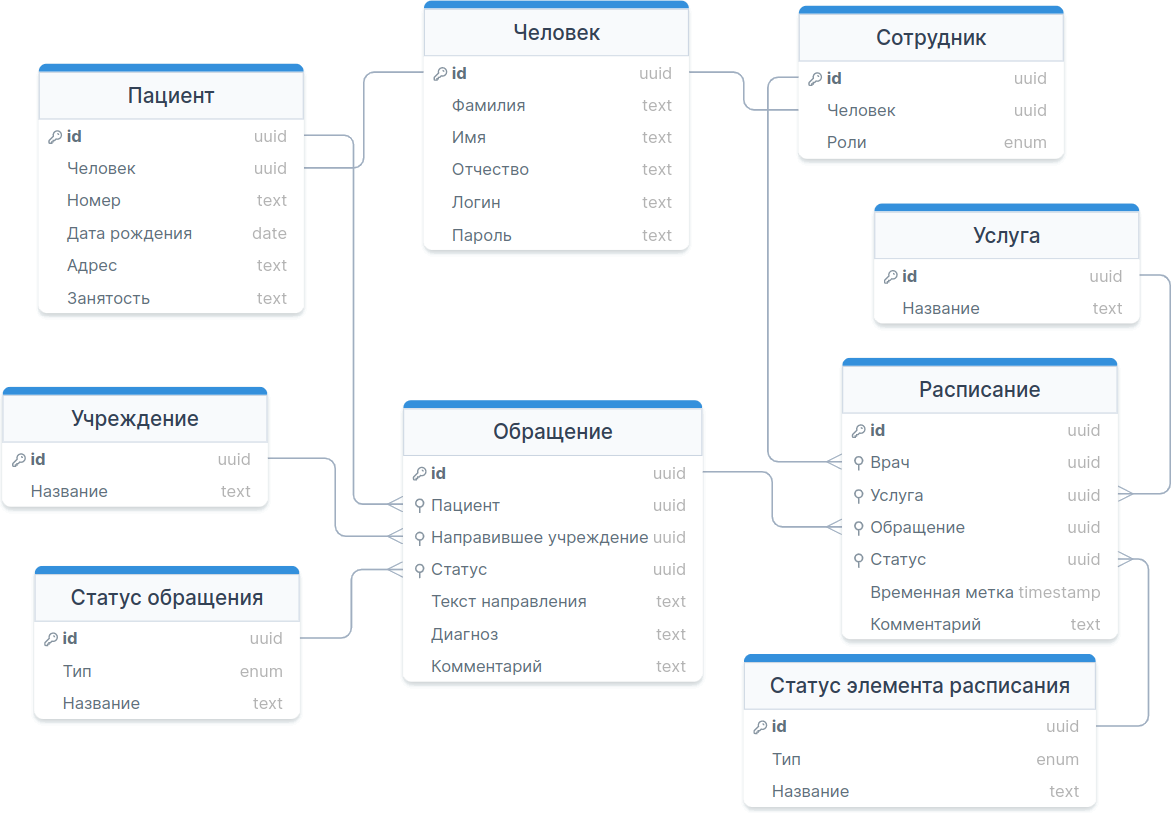
\includegraphics[width=0.9\linewidth]{Логическая схема данных.png}

        \caption{\centering Логическая схема данных}

        \label{fig:Логическая схема данных}

    \end{figure}

    \newpage

    \subsection{Серверная часть}

    Клиентский код не должен напрямую обращаться к базе данных. Ему нужно промежуточное звено - сервер. Передавать данные клиент и сервер должны заранее определённым способом - API. Данные между клиентом и сервером передаются в формате, понятном обоим элементам. После преобразования данных в сущности, сервер работает напрямую с бд. Архитектура серверной части представлена на Рисунке~\ref{fig:Архитектура серверной части}

    \begin{figure}[h]

        \centering

        
\includegraphics[width=0.9\linewidth]{Архитектура серверной части.png}

        \caption{\centering Общая архитектура серверной части}

        \label{fig:Архитектура серверной части}

    \end{figure}

    \subsubsection{Выбор вида API}

    В зависимости от потребностей системы можно использовать разные виды API. Сравнение популярных видов API представлено в Таблице~\ref{tab:Популярные виды API}.

    \begin{xltabular}{\textwidth} { |
            >{\hsize=0.20\hsize} X |
            >{\hsize=0.40\hsize} X |
            >{\hsize=0.40\hsize} X | }
        \hline
        Название
        & Плюсы
        & Минусы \\
        \hline
        REST
        & -- Простота \newline -- Универсальность \newline -- Поддержка CRUD \newline -- Не сохраняет состояние (легко масштабируется)
        & -- Отсутствие строго стандарта \newline -- Низкая производительность при большом количестве запросов \\
        \hline
        SOAP
        & -- Безопасность \newline -- Поддержка транзакций \newline -- Строгий стандарт
        & -- Большая избыточность данных \newline -- Сложность использования и настройки \\
        \hline
        GraphQL
        & -- Нет избыточных данных \newline -- Возможность сложных запросов \newline -- Сильная типизация
        & -- Сложность разработки \newline -- Сложность масштабирования \newline -- Перегрузка из-за сложности запросов \\
        \hline
        gRPC
        & -- Быстрое выполнение \newline -- Сильная типизация
        & -- Сложность в настройке и использовании \\
        \hline
        JSON-RPC и XML-RPC
        & -- Простота использования и разработки \newline -- Лёгкость интеграции
        & -- Нет поддержки HTTP-методов \newline -- Затруднение масштабирования \\
        \hline

        \caption{\centering Популярные виды API}

        \label{tab:Популярные виды API}
    \end{xltabular}

    Для разработки был выбран REST. Его минусы в рамках проекта незначительны: в системе не будет большого количества запросов, а отсутствие строгого стандарта всего лишь делает его принципы рекомендациями. При этом REST удовлетворяет всем потребностям приложения - поддержка HTTP-методов, отсутствие сохранения состояния.

    \subsubsection{Авторизация}

    \begin{xltabular}{\textwidth} { |
            >{\hsize=0.20\hsize} X |
            >{\hsize=0.40\hsize} X |
            >{\hsize=0.40\hsize} X | }
        \hline
        Название & Плюсы & Минусы \\
        \hline
        Basic Auth
        & -- Хорошо работает с HTTPS \newline -- Не требует сессий \newline -- Прост в реализации
        & -- Нет средств управления сессиями \newline -- Передача данных в незашифрованном виде \\
        \hline
        Digest Auth
        & -- Безопасность из-за хеширования для передачи данных
        & -- Сложность реализации \newline -- Нет управления сессиями \\
        \hline
        Token-based Auth \newline (JWT, OAuth)
        & -- Есть управление сессиями \newline -- Передача метаданных
        & -- Сложная реализация и управление токенами \newline -- Проблемы при больших объёмах данных \\
        \hline
        Session-based Auth
        & -- Управление сессиями \newline -- Сервер контролирует данные сессии
        & -- Хранение и управление данными сессии \newline -- Плохо масштабируется \\
        \hline

        \caption{\centering Популярные виды API}

        \label{tab:Популярные виды API}
    \end{xltabular}

    Для данного проекта была выбрана Basic Auth, потому что он прост в реализации. Его проблема безопасности решается использованием HTTPS и он хорошо подходит для проектов небольшого масштаба.

    Заголовок авторизации - специальная строка, передающаяся вместе с запросом. Выглядеть строка должна так: <<Authorization: Basic *токен*>>, где *токен* - Это зашифрованная с помощью Base64 строка вида <<*логин*:*пароль*>>. При запуске приложения создаётся аккаунт по умолчанию, поэтому для всех методов, кроме установки пароля, потребуется авторизация.

    \subsubsection{Методы API}

    Каждый запрос на сервер в разрабатываемой системе характеризуется несколькими параметрами:

    \begin{itemize}[nolistsep]
        \item URL
        \item Метод HTTP
        \item Заголовок авторизации
        \item Параметры в теле запроса, либо в URL
    \end{itemize}

    Зная эти данные мы можем дать нужный ответ. Теперь нужно определить - кто к каким конечным точкам должен иметь доступ. Для этого нужно составлять таблицы с указанием приведённых выше параметров. Поскольку полное расписывание API займёт очень много места, здесь будет приведён сокращённый вариант - без тел запроса. Подробный вариант можно найти в приложении.

    Хорошей практикой считается разделение версий API и выделение его в URL. Поэтому перед каждой конечной точкой в реальных запросах к API дополнительно используется /api/v1, если не сказано иное. Спроектированные методы API представлены в Таблице~\ref{tab:Методы API}

    \begin{xltabular}{\textwidth} { |
        >{\hsize=0.25\hsize} X |
        >{\hsize=0.20\hsize} X |
        >{\hsize=0.55\hsize} X | }

        \hline
        URL & HTTP метод & Краткое описание \\

        \hline
        /people/\{id\}
        & GET, PUT, DELETE
        & Получение, изменение, удаление общих данных о человеке \\

        \hline
        /people/me
        & PUT, GET
        & Получение, изменение данных о себе \\

        \hline
        /people
        & POST, GET
        & Получение списка всех пользователей \\

        \hline
        /patients/\{id\}
        & GET, PUT, DELETE
        & Получение, изменение, удаление пациента \\

        \hline
        /patients
        & POST, GET
        & Получение списка всех пациентов \\

        \hline
        /employees/\{id\}
        & GET, PUT, DELETE
        & Получение, изменение, удаление сотрудника \\

        \hline
        /employees
        & POST, GET
        & Получение списка всех сотрудников \\

        \hline
        /institutions/\{id\}
        & GET, PUT, DELETE
        & Получение, изменение, удаление учреждения  \\

        \hline
        /institutions
        & POST, GET
        & Получение списка всех учреждений \\

        \hline
        /appointments/\{id\}
        & GET, PUT, DELETE
        & Получение, изменение, удаление обращения \\

        \hline
        /appointments
        & POST, GET
        & Получение списка всех обращений \\

        \hline
        /schedules/\{id\}
        & GET, PUT, DELETE
        & Получение, изменение, удаление элемента графика \\

        \hline
        /schedules
        & POST, GET
        & Получение списка всех элементов графика \\

        \hline

        \caption{\centering Методы API}

        \label{tab:Методы API}
    \end{xltabular}

    Отдельно стоит выделить таблицы, к которым должен иметь доступ только администратор. Это такие таблицы, которые меняются очень редко и их изменение сильно влияет на всю систему. Например, изменение в таблице <<Услуги>>. Перечень методов, доступных только Администратору представлен в Таблице~\ref{tab:Методы API только для Администатора}.

    \begin{xltabular}{\textwidth} { |
        >{\hsize=0.34\hsize} X |
        >{\hsize=0.18\hsize} X |
        >{\hsize=0.47\hsize} X | }

        \hline
        URL
        & HTTP метод
        & Краткое описание \\

        \hline
        /procedures/\{id\}
        & GET, PUT, DELETE
        & Получение, изменение, удаление услуги \\

        \hline
        /procedures
        & POST, GET
        & Добавление услуги, получение всех услуг \\

        \hline
        /appointmentStatuses/\{id\}
        & GET, PUT, DELETE
        & Получение, изменение, удаление статуса обращения \\

        \hline
        /appointmentStatuses
        & POST, GET
        & Добавление статуса обращения, получение всех статусов обращений \\

        \hline
        /scheduleStatuses/\{id\}
        & GET, PUT, DELETE
        & Получение, изменение, удаление статуса элемента графика \\

        \hline
        /scheduleStatuses
        & POST, GET
        & Добавление статуса элемента графика, получение всех статусов элементов графика \\

        \hline

        \caption{\centering Методы API только для Администатора}

        \label{tab:Методы API только для Администатора}
    \end{xltabular}

    \subsubsection{Обработка ошибок}\label{Проектирование сервера. Обработка ошибок}

    Обработку ошибок можно разделить на 2 больших пункта:

    \begin{itemize}[nolistsep]
        \item На стороне сервера. Рассмотрим сейчас
        \item На стороне клиента. Будет рассматриваться в пункте~\ref{Проектирование клиента. Обработка ошибок}
    \end{itemize}

    \paragraph{Обработка ошибок базы данных}

    Отдельно выделяются ошибки, связанные с базой данных. Это такие ошибки, которые может быть сложно, либо затратно обнаружить и обработать. Это связано с тем, что база данных - отдельная часть системы, с которой взаимодействует сервер. Есть несколько основных моментов, которые стоит затронуть:

    \begin{itemize}[nolistsep]
        \item \textbf{Транзакционность.} База данных хранит данные - это её основная задача. Контроль корректности вводимых данных на её стороне возможен либо частичный (ограничиваясь, напримар, уникальностью полей), либо очень затратен в создании и поддержке (триггеры). Если данные записались в базу данных, то может быть проблемой удалить их. Особенно это актуально при одновременном создании множества объектов, когда может выполниться только часть запросов. В таких случаях помогает транзакционность - возможность отменить все изменения в рамках связанных запросов. В рамках разрабатываемой системы необходимо учитывать это на стороне сервера.
        \item \textbf{Определение конкретного места ошибки.} Стандартные ошибки, выдаваемые базой данных, не всегда информативны для пользователя, а иногда и для администратора. Так, например, нарушение связи один к одному, либо конфликт из-за уникальности - разные ошибки и их нужно по-разному идентифицировать.
    \end{itemize}

    \paragraph{Коды ошибок}\label{Проектирование сервера. Коды ошибок}

    Сопоставление каждой возможной ошибке конкретного кода может значительно ускорить процесс её обработки. Невозможно заранее знать все возможные причины ошибок - тогда бы их просто не было. Но вполне осуществимо выявление части программы, в которой произошла ошибка. Например, есть код, отвечающий за чтение Person из базы данных. Если мы пометим эту часть кода как вызывающую ошибку с кодом drp-01, то при её возникновении заранее будет известно её расположение. Конечно, это не отменяет вспомогательных сообщений и логирования - лишь помогает им. Список определённых кодов ошибок достаточно большой, их список приведён в Приложении~\{TODO\}.

    \paragraph{Единый формат ошибок}

    Стандартные форматы ошибок могут отличаться от фреймворка к фреймворку, что уменьшает гибкость приложения. Дополнительно, не каждый формат ошибок подходит для каждого приложения - в некоторых много избыточной информации, в некоторых её недостаточно. Поэтому для приложения был разработан единый формат ошибок, использующий JSON. Представлен на Рисунке~\ref{fig:Формат ошибок}.

    \begin{figure}[h]

        \centering

        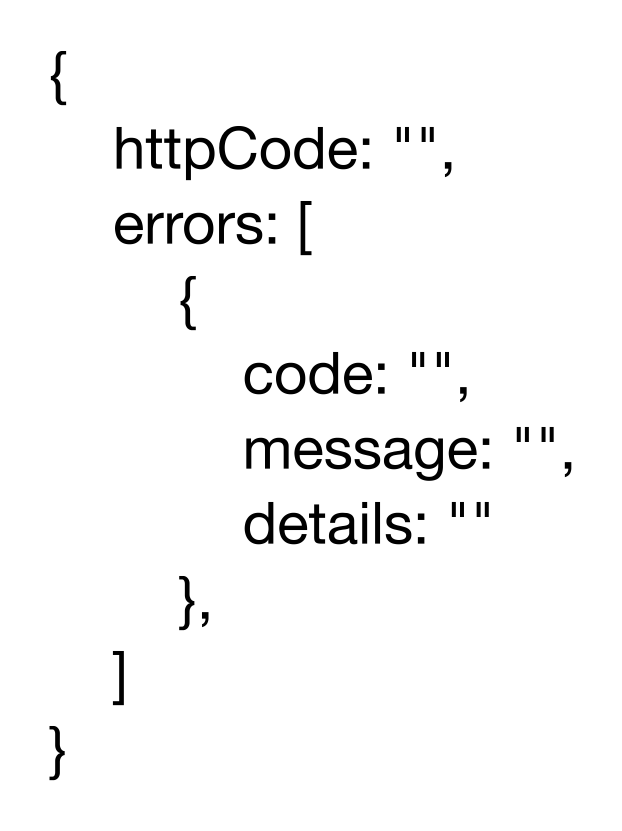
\includegraphics[width=0.3\linewidth]{Формат ошибок.png}

        \caption{\centering Формат ошибок}

        \label{fig:Формат ошибок}

    \end{figure}

    Разберём по частям:

    \begin{itemize}[nolistsep]
        \item \textbf{httpCode.} У протокола http есть перечень поддерживаемых кодов состояния. Например, коды 2XX - коды успешного выполнения запрося, 4XX - ошибки клиента, 5XX - ошибки сервера. Это общепринятые заданные стандартом коды. Здесь потребуются только коды, отвечающие за ошибки. Явное указание кода в ответе упрощает работу с ошибкой при отладке.
        \item \textbf{errors.} Массив ошибок. Перечень того, что сервер в процессе обработки запроса посчитал некорректным. Стоит отметить, что перечисляются не все ошибки, а лишь те, до которых сервер обработал данные. Несколько элементов может быть указано только если ошибки одного типа, например, все касаются валидации полей.
        \begin{itemize}[nolistsep]
            \item \textbf{code.} Внутренний код ошибки системы, определённый в пункте~\ref{Проектирование сервера. Коды ошибок}.
            \item \textbf{message.} Написанное доступным простому пользователю языком сообщение об ошибке, выводимое на экран.
            \item \textbf{details.} Более развёрнутое сообщение об ошибке, содержащее максимум данных для отладки. Опциональное поле.
        \end{itemize}
    \end{itemize}

    \newpage

    \subsection{Клиентская часть}

    Клиентская часть завершает список необходимых компонентов для клиент-серверного приложения. Это та часть, которую пользователь видит на экране. Сюда, по большей части, относится графический интерфейс и работа с ним. Сюда же входит работа с API сервера: формирование запросов, обработка ответов.

    \subsubsection{Архитектура клиентского приложения}

    Для разработки понадобятся различные компоненты, такие как диалоговые окна, кнопки, элементы для поиска элементов. Рассмотрим, какие компоненты нужны для работы системы:

    \textbf{Поля ввода.} На первый взгляд, это один компонент. Но для удобной работы нужно детализировать его для разных нужд:

    \begin{itemize}[nolistsep]
        \item Обычные поля, не требующие особого подхода. Например, комментарий к обращению может быть написан в свободной форме.
        \item Пароль. Требует сокрытия вводимых данных.
        \item Поля со строго определённой структурой. Необходимы для, например, наглядного ввода номера телефона
    \end{itemize}

    Кроме того, большинство полей в базе данных приложения требуют гарантии заполненности. Так услуга не имеет смысла без её названия. Нужна возможность визуальных подсказок для полей.

    \textbf{Алерты.} Компоненты, информирующие пользователя о событиях. Когда на странице не могут загрузиться данные, либо произошла какая-то ещё ошибка, то нужно об этом сказать пользователю. Для этого хорошо подходит отдельный компонент.

    \textbf{Выпадающие списки.} Заменяют поля ввода, когда список его значений заранее известен и достаточно мал.

    \textbf{Диалоговые окна.} Это элементы, появляющиеся поверх основной страницы и служащие для совершения какого-то фиксированного действия. Например, отправка запроса на создание элемента или выбор элемента из множества на основе фильтров. В разделе~\ref{Техническое задание} упоминалось, что в системе будет Администратор. Он должен иметь возможность редактировать все записи в базе данных. Для этого ему потребуется диалоговое окно на куждую из сущностей. Они же будут использоваться и для остальных ролей в случаях, когда доступ к сущностям есть.

    \subsubsection{Проектирование интерфейса пользователя}

    В пункте~\ref{Техническое задание} выделено 4 роли: Пациент, доктор, регистратор, администратор. У каждого из них, в соответствии с пунктами~\ref{ТЗ. Пациент}~-~\ref{ТЗ. Администратор} в системе свои возможности. Для этого необходимо разграничение интерфейса. Роли с указанием доступных им страниц представлены в Таблице~\ref{tab:Роли в системе и доступные им страницы}

    \begin{xltabular}{\textwidth} { |
        >{\hsize=0.30\hsize} X |
        >{\hsize=0.70\hsize} X | }

        \hline
        Роль
        & Доступные страницы \\

        \hline
        Пациент
        & - Просмотр расписания врача \newline - Подача заявки на приём \\

        \hline
        Доктор
        & - Запись к себе \newline - Создание своего расписания \newline - Просмотр расписаний других врачей \\

        \hline
        Регистратор
        & - Расписания врачей \newline - Пациенты \\

        \hline
        Администратор
        & - Страницы с доступом для редактирования для каждой сущности \\

        \hline

        \caption{\centering Роли системы и доступные им страницы}

        \label{tab:Роли в системе и доступные им страницы}
    \end{xltabular}

    \subsubsection{Обработка ошибок}\label{Проектирование клиента. Обработка ошибок}

    Важная часть разработки клиентского приложения - правильная обработка ошибок. Она помогает предотвратить прерывание работы приложения, выявить и устранить причину ошибок. Продуманная система обработки ошибок важна для стабильности приложения.

    Существуют разные виды ошибок, которые должно обрабатывать клиентская сторона, например:

    \begin{itemize}[nolistsep]
        \item Обработка ошибок на уровне приложения
        \item Ошибки, генерируемые сервером. Например, запрос недоступного пользователю ресурса
        \item Некорректный ввод пользователя. Частично относится к прошлому пункту, но выделение позволяет сделать интерфейс удобнее
        \item Недоступность сервера
    \end{itemize}

    Подробнее рассмотрим важные элементы обработки ошибок

    \paragraph{Валидация данных}\label{Проектирование клиента. Валидация данных}

    Для предотвращения ошибок, связанных с неверными данными, в приложении необходимы механизмы проверки ввода - валидации. Это включает валидацию свойств компонентов, использование библиотек для валидации форм и других пользовательских данных посредством специальных заранее определённых правил.

    \paragraph{Логирование ошибок}

    Для упрощения отладки и мониторинга работы приложения необходимо использовать систему логирования ошибок. Она включает вывод и сохранение информации об ошибках, отправку данных об ошибках на сервер. Важно одновременно и уведомлять пользователя об ошибках, и сохранять данные о них, поскольку это разные уровни взаимодействия. Первые события рассчитаны больше на пояснение того, что случилось, в понятной простому человеку форме, а вторые - на то, что их будет разбирать специалист, для чего нужно сохранять больше информации.

    \paragraph{Обработка ошибок в пользовательском интерфейсе}

    Информативные сообщения об ошибках и уведомлениях в пользовательском интерфейсе улучшают пользовательский опыт. Основная реализация - всплывающие подсказки и уведомления. Стоит затронуть и необходимость визуального выделения ошибок, казающихся валидаций данных из пункта~\ref{Проектирование клиента. Валидация данных}.

    \newpage

    \section{Реализация}\label{Реализация}

    \subsection{Выбор технологий}\label{Реализация. Выбор}

    Выбор инструментов реализации проводится параллельно с проектированием. Это начальный этап разработки, который может определять структуру системы. В пункте~\ref{Проектирование} указано, что частей системы 3: база данный, серверная и клиентские части. Рассмотрим реализацию каждой из них.

    \subsubsection{База данных}\label{Реализация. Выбор. База данных}

    Изначальное условие для системы было -- использование СУБД Oracle. Если разработанная система будет внедряться, то чтобы не было конфликтов в базе данных. Потому что разные СУБД имеют разные ограничения на имена, например, на длину и заререзрвированные слова. Забегая вперёд -- вся работа с базой данных будет через спецификацию JPA, то есть смена СУБД почти не потребует затрат.

    \subsubsection{Серверная часть}\label{Реализация. Выбор. Серверная часть}

    При выборе технологического стека для сервернои части важно учитывать такие требования, как производительность, стабильность, безопасность, масштабируемость. Сравнение основных стеков представлено в Таблице~\ref{tab:Сравнение технологических стеков для серверной части}.

    \begin{xltabular}{\textwidth} { |
        >{\hsize=0.30\hsize} X |
        >{\hsize=0.70\hsize} X | }

        \hline
        Состав стека
        & Особенности \\

        \hline
        Java + Spring
        & -- Высокая производительность и скорость выполнения \newline -- Хорошая интеграция с Oracle Database \newline -- Богатый набор библиотек для различных задач \newline -- Строгая статическая типизация для повышения надежности кода \newline -- Многопоточная модель, подходящая для CPU-интенсивных операций и масштабируемых систем \\

        \hline
        Python + Django
        & -- Скорость разработки \newline -- Много функций "из коробки" \newline -- Динамическая типизация \newline -- Меньшая производительность по сравнению с Java \newline -- Интеграция с Oracle может быть менее гибкой \\

        \hline
        JavaScript + Node.js
        & -- JavaScript на сервере и клиенте, упрощая разработку \newline -- Однопоточная модель с асинхронной I/O, эффективной для обработки большого количества коротких запросов \newline -- Низкая производительность для CPU-интенсивных операций по сравнению с Java \newline -- Динамическая типизация и возможные проблемы безопасности \\

        \hline

        \caption{\centering Сравнение технологических стеков для серверной части}

        \label{tab:Сравнение технологических стеков для серверной части}
    \end{xltabular}

    \subsubsection{Клиентская часть}\label{Реализация. Выбор. Клиентская часть}

    У клиентский части приложения большое количество нюансов, которые нужно учесть. Они связаны с тем, что этот код будет выполняться на разных компьютерах и нужно обеспечить корректную работу на них.

    Основной язык разработки -- JavaScript. TypeScript -- разработанный компанией Microsoft язык, расширяющий возможности TypeScript: обладает статической типизацией, поддержкой полноценныз классов. К тому же он совместим с JavaScript. Он повышает читаемость кода, его повторное использование и скорость поиска ошибок.

    JavaScript отвечает за внутреннюю логику, за внешний вид отвечает HTML и CSS. Можно писать код используя только их, но такой подход хорош только для очень маленьких приложений. Так, работу на разных экранах придётся обеспечивать вручную. Как и следить за цветовой палитрой, стилями и анимацией. Гораздо удобнее использовать фреймворки, так как они представляют готовый набор стандартных элементов и логики. Популярных фреймворка 3:

        \begin{itemize}[nolistsep]
        \item \textbf{React.} Гибкий, с большим количеством библиотек, но для полноценной разработки именно потребуется использование сторонних библиотек, что может быть затруднением.
        \item \textbf{Angular.} Большой фреймворк со всеми нужными компонентами из коробки, чёткая структура, но сложный для изучения и малопроизводительный.
        \item \textbf{Vue.js.} Гибкий, самодостаточный фреймворк с возможностью интеграции со сторонними библиотеками. Прост в освоении, хорошая документация, но меньше материала по сравнению с другими.
    \end{itemize}

    С Vue.js я работал и это, пожалуй, лучший выбор для данной системы. Приложению не нужны супермасштабы и встроенных инструментов хватит для разработки приложения.

    \subsection{База данных}\label{Реализация. База данных}

    \subsection{Серверная часть}\label{Реализация. Серверная часть}

    \subsection{Клиентская часть}\label{Реализация. Клиентская часть}

    \newpage

    \section*{Заключение}
    \addcontentsline{toc}{section}{Заключение}

    \newpage

    \addcontentsline{toc}{section}{Список использованных источников}

    \begin{thebibliography}{}
        \bibitem{natsproektzdravoohranenie} Федеральный проект <<Создание единого цифрового контура в здравоохранении на основе единой государственной информационной системы в сфере здравоохранения (ЕГИСЗ)>> - 2019 - 9 августа [Электронный ресурс] - URL: \url{https://minzdrav.gov.ru/poleznye-resursy/natsproektzdravoohranenie/tsifra/} (Дата обращения: 13.12.2022)
        \bibitem{apiwikipedia} Википедия. API - 2023 [Электронный ресурс] - URL: \url{https://ru.wikipedia.org/wiki/API} (Дата обращения: 20.01.2023)
    \end{thebibliography}

\end{document}
